\documentclass{beamer}
\beamertemplatenavigationsymbolsempty
\usecolortheme{rose}
\setbeamertemplate{blocks}[rounded=true, shadow=true]
\setbeamertemplate{footline}[page number]
%
\usepackage[utf8]{inputenc}
\usepackage[english, russian]{babel}
\usepackage{amssymb,amsfonts,amsmath,mathtext}
\usepackage{subfig}
\usepackage{graphicx}
\usepackage[most]{tcolorbox}
\usepackage[all]{xy} % xy package for diagrams
\usepackage{array}
\usepackage[dvipsnames]{xcolor}
\usepackage{multicol}% many columns in slide
\usepackage{hyperref}% urls
\usepackage{multirow}
\usepackage{hhline}%tables
% Your figures are here:
\graphicspath{ {fig/} {../fig/} }
\usepackage{ragged2e}
\justifying
\documentclass{amsart}
\definecolor{skyblue}{rgb}{0.75, 0.87, 0.93}

\newcommand{\vx}{\mathbf{x}}
\newcommand{\vh}{\mathbf{h}}
\newcommand{\vf}{\mathbf{f}}
\newcommand{\vW}{\mathbf{W}}
\newcommand{\vb}{\mathbf{b}}
%----------------------------------------------------------------------------------------------------------
\title{{Анализ неопределенности и внутренних представлений языковых моделей для поиска сгенерированных документов}}
\author{
    Анастасия Евгеньевна Вознюк\\
    Научный руководитель: к.ф.-м.н. А.\,В.\,Грабовой
}
\date{18 мая 2024 г.}
\institute[МФТИ (НИУ)]{
    Кафедра интеллектуальных систем ФПМИ МФТИ\\
    Специализация: Интеллектуальный анализ данных\\
    % Направление: 01.03.02 Прикладные математика и информатика\\
}
\date{\footnotesize
% \par\smallskip\emph{Научный руководитель:} Андрей Грабовой
\par\bigskip\small 17 мая 2024}

%----------------------------------------------------------------------------------------------------------
\begin{document}
%----------------------------------------------------------------------------------------------------------
\begin{frame}
\thispagestyle{empty}
\maketitle
\end{frame}
%-----------------------------------------------------------------------------------------------------
\begin{frame}{Цель работы}

Исследуется проблема поиска машинно-сгенерированных документов. Стандартные методы поиска не являются устойчивыми к смене генератора или смене домена, поэтому нужно предложить более устойчивые методы.

Предлагается исследовать методы анализа внутренних представлений языковых моделей, а также внутренних размерностей текстов при обработке текстового документа. 

Кроме того, дополнительной сложностью является смешение авторов в документе уже не на уровне фрагментов но на уровне небольших изменений.



\end{frame}
%----------------------------------------------------------

\begin{frame}{Общая постановка задачи}
Определим документ как конечную последовательность символов из заданного алфавита $\mathbf{W}$. Пространство документов:
$$\mathbb{D} = \Bigl\{\Big[t_j\Big]_{j=1}^n \quad|\quad t_j \in \mathbf{W}, n \in \mathbb{N}\Bigr\}.$$

Дан набор из $N$ документов
$$\mathbf{D} = \bigcup_{i=1}^{N}D^i, D^i \in \mathbb{D}.$$

Определим множество авторов, тексты которых встречаются в наборе $\mathbf{D}$:
$$\mathbf{C} = \{0, \dots, k - 1\}.$$


Тогда задача классификации автора документа записывается как: 
\begin{equation}
    \mathbf{\phi}: \mathbb{D} \rightarrow \mathbf{C}
\end{equation}
\end{frame}



\begin{frame}{Задача 1: Деткция преобразований текстов документов}
    Определим два операции:
    \begin{enumerate}
        \item Удалить $\text{DELETE}(D, i_{\text{start}}, i_{\text{end}}) = D_{<i_{\text{start}}}\cdot D_{>i_{\text{end}}}$
        \item Вставить $\text{INSERT}(D, t, i_{\text{start}}) = D_{<i_{\text{start}}}\cdot t\cdot  D_{\geq i_{\text{start}}}$
    \end{enumerate}
    Любые преобразования над текстом можно выразить через эти две операции. Так, самыми распространенными операциями являются: а)~\textit{Polish}, б)~\textit{Complete}, в)~\textit{Rewrite}.

    Для экспериментов был взят датасет искуственных текстов с различными дополнительными преобразованиями RAID\footnote{RAID: A Shared Benchmark for Robust Evaluation of Machine-Generated Text Detectors}.
\end{frame}

% \begin{frame}{Детекция фрагментов в документе}
% Для каждого документа $d \in \mathbb{D}$ существует представление в виде разбиения на фрагменты различного авторства:
% $$ \mathbb{T} = \Bigl\{\Big[t_{s_j}, t_{f_j}, C_j\Big]_{j = 1}^{J} \quad|\quad t_{s_j} = t_{f_{j - 1}},\quad s_j \in \mathbb{N}_0,\quad f_j \in \mathbb{N}, \quad C_j \in  \mathbf{C} \Bigr\},$$

% где $J$ - количество фрагментов разного авторства в документе, $t_{s_j}$ и $t_{f_j}$ - начало и конец $j$-ого фрагмента, внутри которого все токены одного авторства, $C_j$ - автор $j$-ого фрагмента. 

% \newline
% Тогда модель детектора определяется как композиция отображений:
% $$\mathbf{\phi}: \mathbb{D} \rightarrow \mathbb{T} \quad \quad \mathbf{\phi} : \mathbf{g} \circ \mathbf{f},$$
% где $\mathbf{f}$~--- отображение для выделения текстовых фрагментов, а $\mathbf{g}$  - отображение для классификации получившихся фрагментов.
% \end{frame}


\begin{frame}{Признаки латентного пространства модели}

% Suggest we have our input context $\textbf{x}$, $y_k = f(\textbf{x}, y_1, \dots, y_{k - 1} |\textbf{\theta})$, $\textbf{y} = [y_1, \dots, y_n]^T$


$\pmb{\theta}$ - параметры нашей модели $f$. 
$$y_k = f(D, y_1, \dots, y_{k - 1} \mid \pmb{\theta})$$
$$\pmb{y} = [y_1, \dots, y_n]^T$$

\textbf{Maxiumum Sequence Probability}
\begin{equation}  
\text{MSP}(\pmb{y} | D, \pmb{\theta}) = 1 -P(\pmb{y} | D, \pmb{\theta})
\end{equation} 


\textbf{Perplexity}
\begin{equation}
P(\textbf{y} | D,  \pmb{\theta}) = \exp\{-\frac{1}{|D|}\log P(\textbf{y} | D, \pmb{\theta})\}
\end{equation} 

\textbf{Mean Token Entropy}
\begin{equation}
\mathcal{H}_T(\mathbf{y}, D ; \boldsymbol{\theta})=\frac{1}{|D|} \sum_{l=1}^{|D|} \mathcal{H}\left(y_l \mid \mathbf{y}_{<l}, D, \boldsymbol{\theta}\right)
\end{equation} 

\end{frame}

\begin{frame}{RQ1: Можно ли разделить между собой тексты с преобразованием и без с помощью этих признаков?}
% First row
    \begin{minipage}{0.48\textwidth}
        \centering
        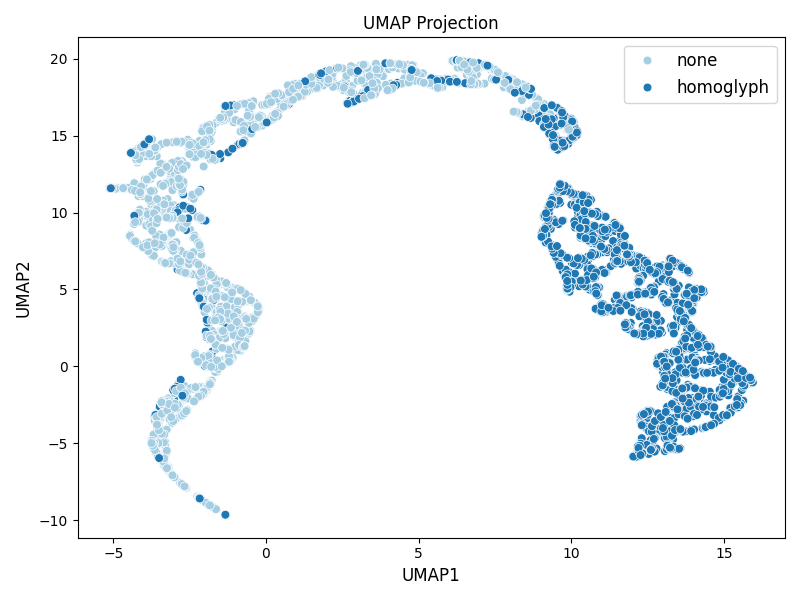
\includegraphics[width=\linewidth]{images_sem2/umap_homoglyph.png}
    \end{minipage}\hfill
    \begin{minipage}{0.48\textwidth}
        \centering
        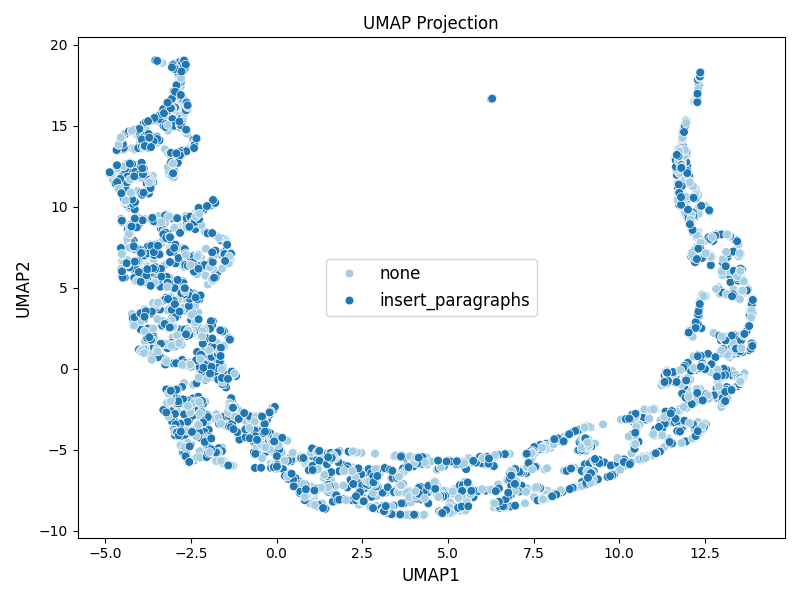
\includegraphics[width=\linewidth]{images_sem2/umap_insert_paragraphs.png}
    \end{minipage}

    \vspace{0.05cm}

    % Second row
    \begin{minipage}{0.48\textwidth}
        \centering
        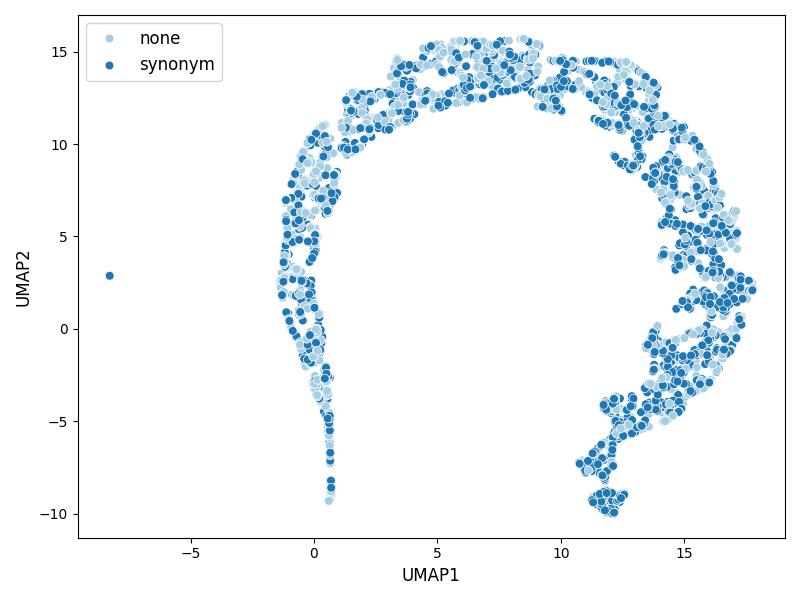
\includegraphics[width=\linewidth]{images_sem2/umap_synonym.png}
    \end{minipage}\hfill
    \begin{minipage}{0.48\textwidth}
        \centering
        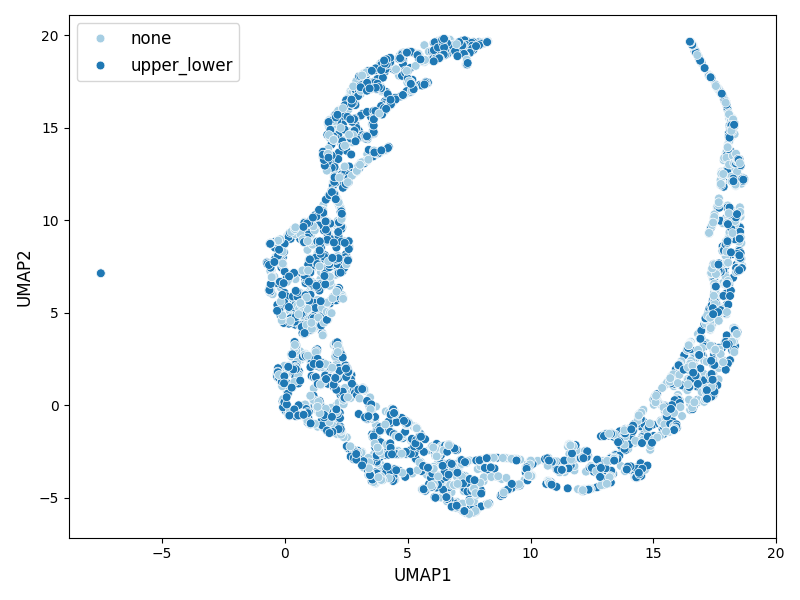
\includegraphics[width=\linewidth]{images_sem2/umap_upper_lower.png}
    \end{minipage}
\end{frame}

\begin{frame}{RQ1: Можно ли разделить между собой тексты с преобразованием и без с помощью этих признаков?}
    \begin{figure}
        \centering
        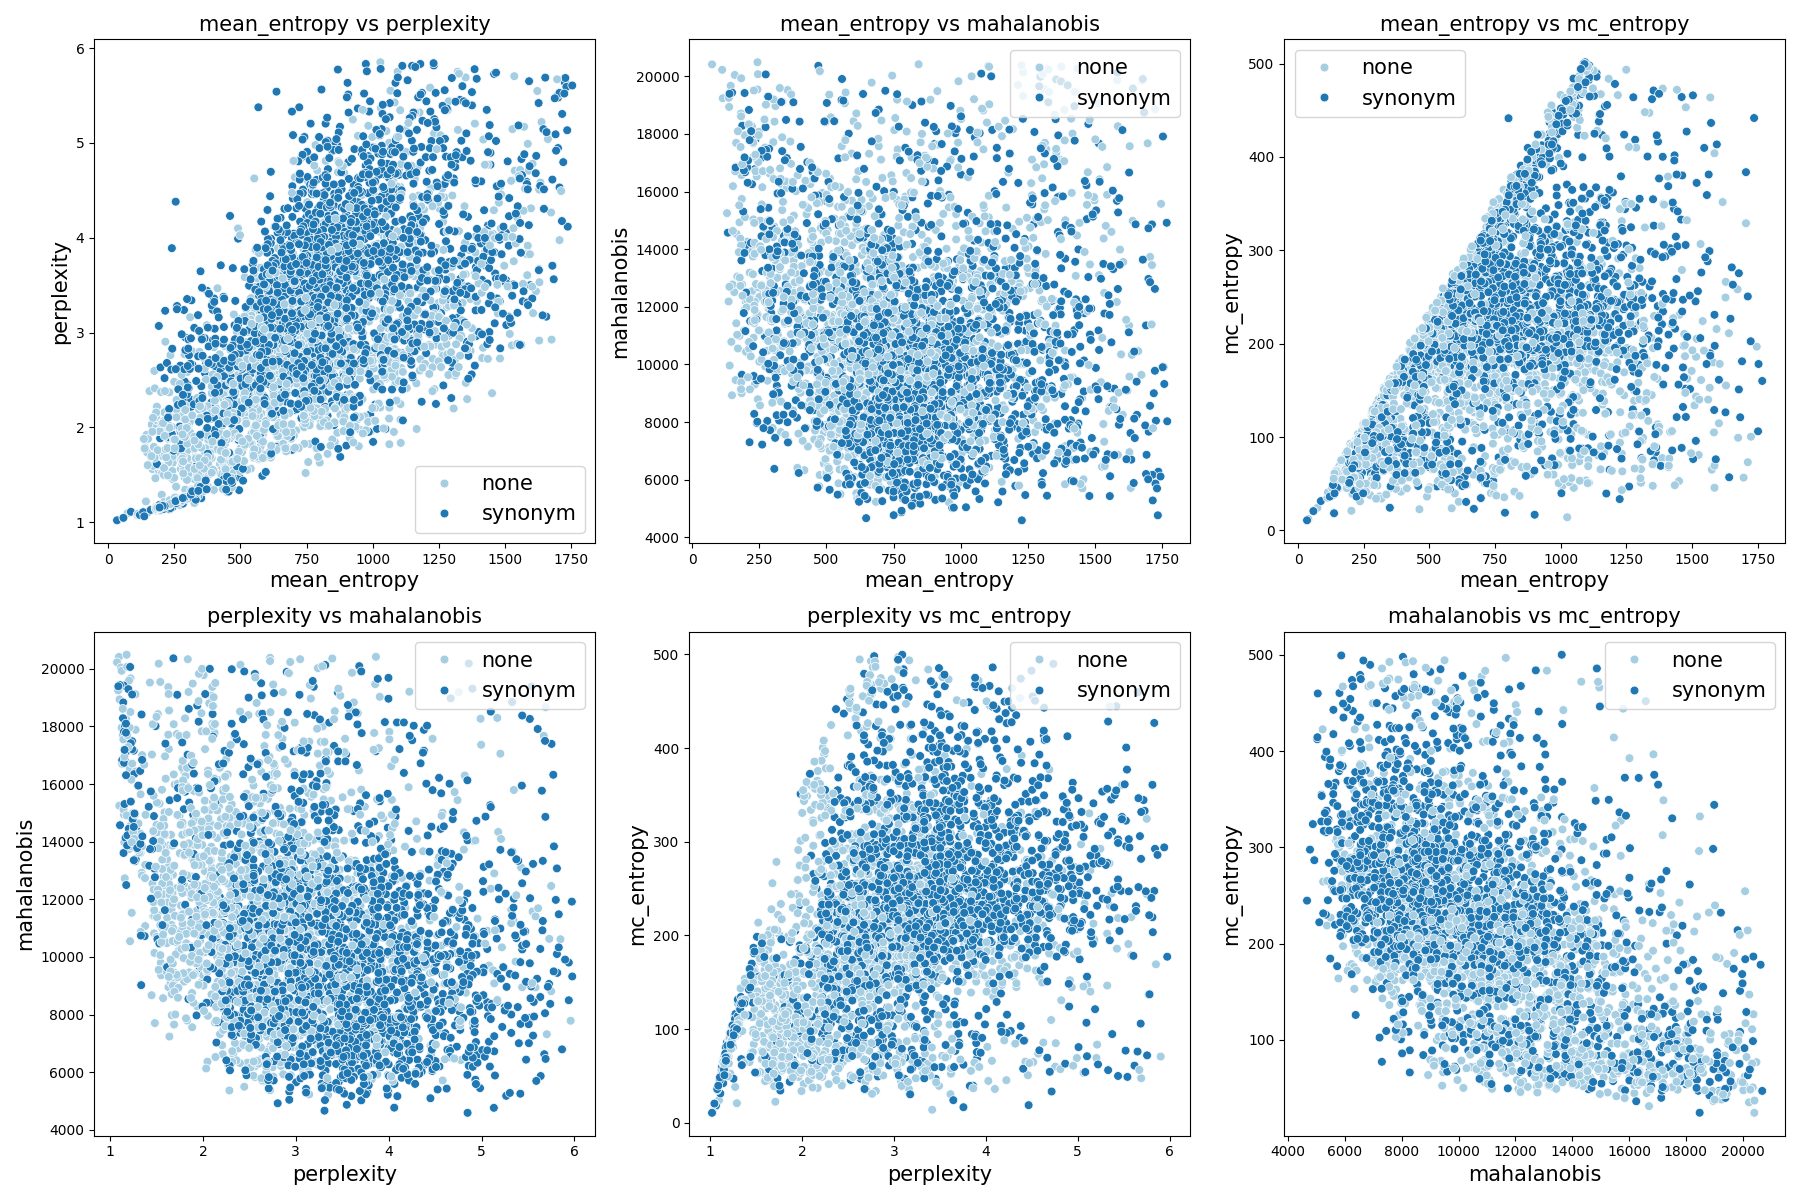
\includegraphics[width=\linewidth]{images_sem2/pairplot.png}
        \label{fig:enter-label}
    \end{figure}
\end{frame}


\begin{frame}{Задача 2: Анализ внутренних представлений}

    \centering
    \begin{minipage}{0.48\textwidth}
        \centering
        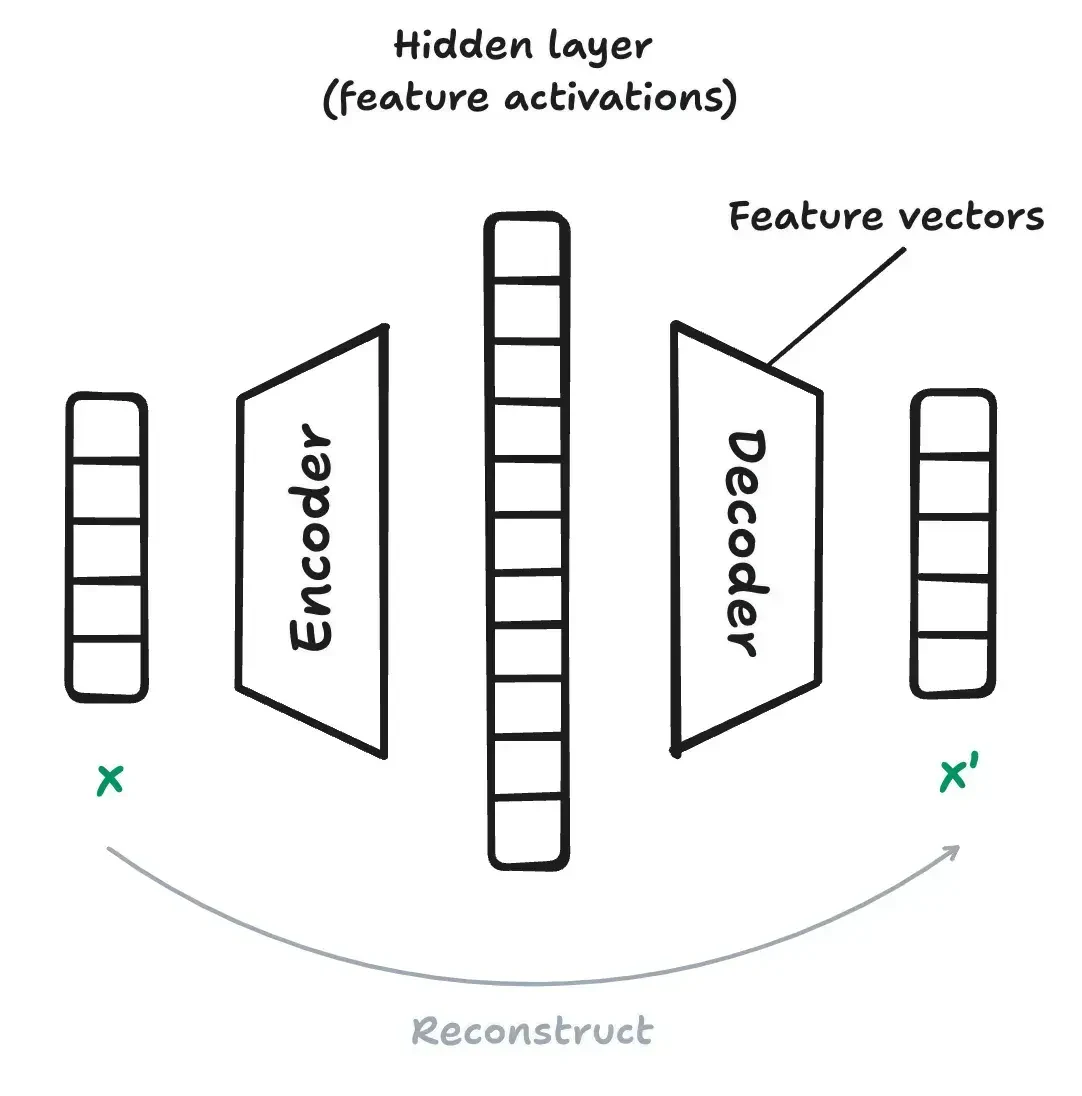
\includegraphics[width=\linewidth]{images_sem2/scheme_sae.png}
    \end{minipage}\hfill
    \begin{minipage}{0.48\textwidth}
        \centering
        Пусть есть активации языковой модели $\vx$, SAE декомпозирует их и потом конструирует обратно с некоторой функцией $\sigma$:
        $$f(\vx) = \sigma(\vW_{\text{enc}} \vx + \vb_{\text{enc}})$$
        $$\hat{x}(f) = \vW_{\text{dec}} f(\vx) + \vb_{\text{dec}}$$
        $\hat{x}(f(\vx))$ -- отображение обратно в $\vx$;
        $f(\vx) \in \mathbb{R}^M$ ($M \gg d$) -- sparse вектор признаков. 
    \end{minipage}

\end{frame}

\begin{frame}{Результаты применения SAE}
    \begin{figure}[t] 
    \centering
    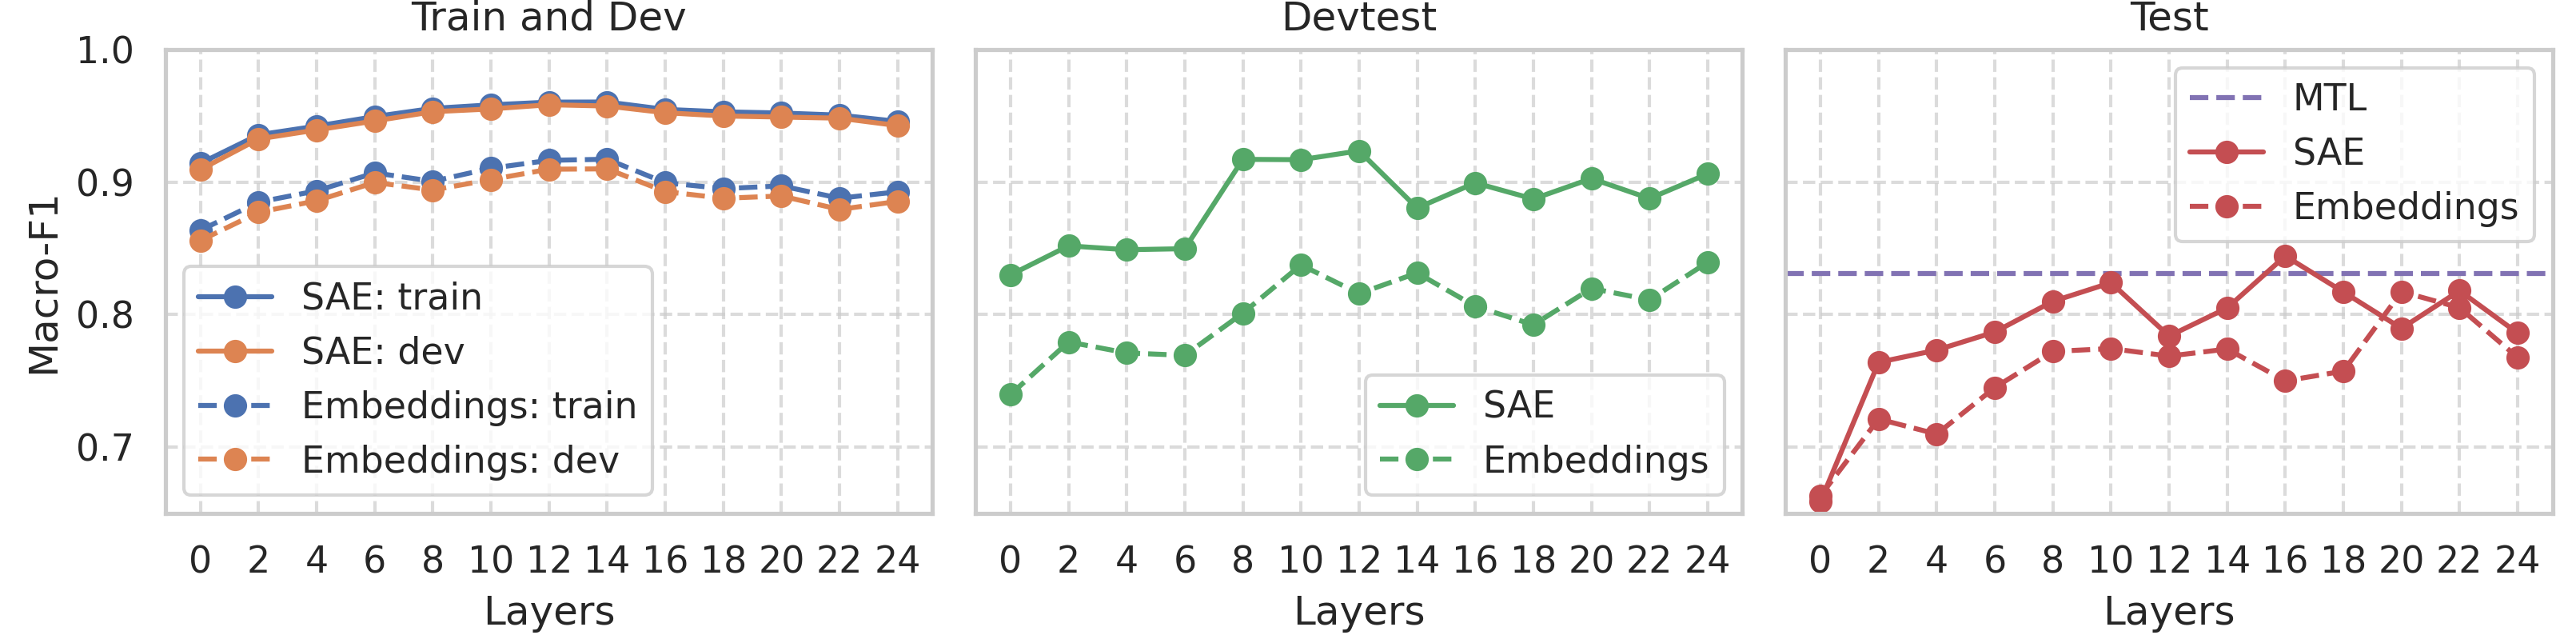
\includegraphics[width=\textwidth]{images_sem2/main_metrics.png} 
    \caption{Macro F1 при обучении XGBoost на внутренних представлениях и признаках, полученных с помощью SAE на различных поднаборам датасета COLING\footnote{Feature-Level Insights into Artificial Text Detection with Sparse Autoencoders}}
    \label{fig:main_metrics}
\end{figure}
\end{frame}
\section{итоги}
\begin{frame}{Итоги НИР за семестр и планы на следующий семестр}
    \begin{block}{Результаты}
    \begin{enumerate}
        \item Принята 1 работа на A конференцию, еще с одной работой было выступление на конференции AAAI;
        \item Проведены эксперименты с подсчетом признаков над латентным пространством для выявления текстовых преобразований;
        \item Получены результаты для применения SAE для детекции искуственных текстов; проведена интерпретация полученных признаков;
    \end{enumerate}
    \end{block}

    \begin{block}{Планы}
    \begin{enumerate}
        \item Применить SAE для различных преобразований над текстами (уже в работе, проводим эксперименты);
    \end{enumerate}
    \end{block}
    
    % \begin{tcolorbox}[colback=white,colframe=skyblue,title=Планы]
    % Можно адаптировать PHD для новых моделей, так что она все еще будет статистической метрикой разделимости текстов.
    % \end{tcolorbox}
\end{frame}

%------------------------------------------------------------------------
% \begin{frame}{Выносится на защиту}
%     \begin{enumerate}
%         \item Архитектура решения для детекции смены авторов в текстах, когда смена авторов происходит только на уровне параграфов (результат осеннего семестра)
%         \item Архитектура решения для детекции смены авторов в тексте, в случае, когда эта смена авторов происходит единожды, но может быть в произвольном токене
%         \item Использование CRF для задачи детекции границ авторов
%     \end{enumerate}
% \end{frame}

\begin{frame}[noframenumbering,plain]{Список работ автора по теме НИР}
        \begin{block}{Препринты}
        \begin{enumerate}
            \item Feature-Level Insights into Artificial Text Detection with Sparse Autoencoders. \textit{принято на ACL Findings 2025}
        \end{enumerate}
    \end{block}
    \begin{block}{Выступления с докладом}
        \begin{enumerate}
            \item Are AI Detectors Good Enough? A Survey on Quality of Datasets With Machine-Generated Texts// \textit{AAAI 2025 Preventing and Detecting LLM Misinformation (PDLM), 3 марта 2025}
        \end{enumerate}
    \end{block}
\end{frame}
%------------------------------------------------------------------------
\end{document} 